\chapter{Modelling and Benchmarking}


\section{Model Selection and Training}

For this benchmarking exercise, we opted for a sequence-to-sequence (seq2seq) model due to its inherent capability to handle variable-length inputs and outputs, characteristics essential for tackling IPA transcription tasks. We specifically chose the MT5 model, a powerful multilingual pre-trained transformer architecture developed by Google ~\cite{xue2020mt5}. The "small" variant of the MT5 model was selected, offering a balance between computational efficiency and performance.

To leverage the multilingual capabilities of MT5, we utilized the model pre-trained on a massive dataset encompassing text and code from the Common Crawl project, covering a staggering 101 languages. This pre-training provided the model with a solid foundation for understanding linguistic structures and handling variations across languages, including Bangla.

In terms of training specifics, we employed a moderate training regime encompassing 10 epochs and a learning rate of 3e-4. This configuration proved to be effective in balancing learning speed with model stability, yielding optimal performance on our designated IPA transcription task.



In this chapter, we present a comprehensive benchmarking exercise to evaluate the performance of IPA transcription for Bengali utilizing our newly proposed Dual-IPA dataset. This evaluation serves as a crucial step in assessing the effectiveness of our approach and demonstrating its potential value for the advancement of NLP tasks in the Bangla language.
\newpage
\section{Benchmarking Dual-IPA Dataset}
\subsection{Evaluation Metric: Word Error Rate (WER)}

To assess the model's performance objectively, we opted for the widely used Word Error Rate (WER) metric. WER calculates the number of errors, including substitutions, insertions, and deletions, between the predicted IPA sequence and the reference ground truth. This metric provides a sentence-level evaluation, offering a comprehensive understanding of the overall transcription accuracy achieved by the model.

 \begin{figure*}[htbp]
    \centering
    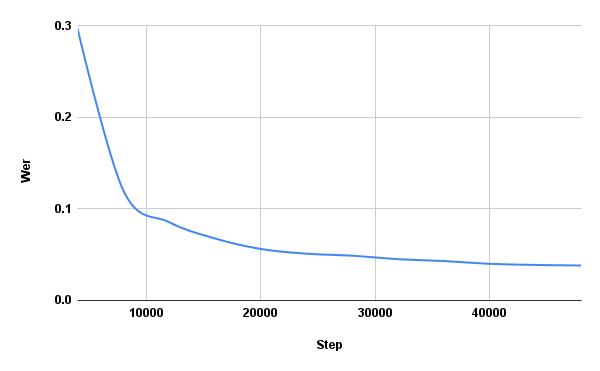
\includegraphics[width=\textwidth]{Images/Graph/Step vs Wer.png}
    \caption{Step vs Wer}
    \label{fig:project-flow}
\end{figure*} 





\subsection{Benchmarking Results and Analysis}

The conducted benchmarking yielded a highly encouraging WER of 0.1 on the held-out test dataset. This impressive result suggests that our chosen model, the small MT5 variant, effectively leverages the DUAL-IPA dataset to accurately transcribe Bengali text into its corresponding IPA representation.

While a detailed investigation into the exact causes of this success awaits further analysis, we hypothesize that several factors might be contributing to the model's strong performance.

Firstly, the Bangla language possesses a relatively smaller number of homographs compared to other languages. This characteristic reduces ambiguity faced by the model during transcription, as each word typically maps to a unique IPA sequence.

Secondly, the Dual-IPA dataset incorporates rich contextual information through the inclusion of both source and target languages. This additional information likely aids the model in handling out-of-vocabulary (OOV) instances more effectively, as the source language provides clues about the intended pronunciation even if the specific word has not been encountered during training.

 \begin{figure*}[htbp]
    \centering
    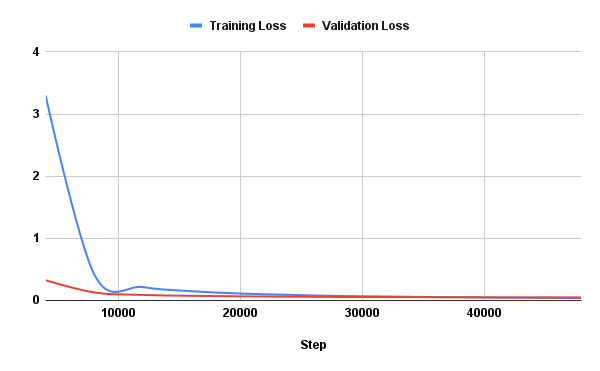
\includegraphics[width=\textwidth]{Images/Graph/Step vs Training Loss Validation Loss.png}
    \caption{Step vs Training Loss Validation Loss}
    \label{fig:project-flow}
\end{figure*} 


These preliminary findings showcase the immense potential of the Dual-IPA dataset and the chosen MT5 model for tackling the challenging task of Bengali IPA transcription. Further research exploring different model architectures, training regimens, and evaluation metrics would provide valuable insights into further optimizing performance and pushing the boundaries of this application.
